
\chapter{Point cloud based methods}
\label{ch:point_cloud_based}

Reconstructing surfaces from point clouds is a lively branch in computational geometry.
As discussed when summarizing the state of the art, \cf \cref{ch:state_of_the_art}, several well-working methods have been developed to convert a set of points into a polyhedral surface, \ie triangle meshes in most cases.
One possible explanation for this richness in algorithms is that point clouds are heavily used for their simplicity when digitizing real-world objects, \eg by scanning their surface with lasers or depth-sensing cameras.

Some algorithms temporarily create intermediate representations, \eg Voronoi diagrams and medial axes, like the cocone \cite{cocone, tight_cocone, robust_cocone} and crust \cite{crust, power_crust} family, or functional ones, like the MLS \cite{mls}, RBF \cite{rbf} or signed distance functions \cite{sdf_surface_reconstruction} approaches.
Thus, some of these algorithms have other uses as well beside surface reconstruction.
Other methods create surface triangles directly, mostly by growing a region on the sampled surface.
These so-called region-growing or advancing front algorithms are typically faster but more susceptible to noisy input, \eg BPA and G2S.
Eventually, this collection of algorithms should also be available for reconstructing surfaces from the VML's data model.

In the previous \cref{ch:tri_dexel}, the tri-dexel based surface reconstruction approach relied on a raycast to sample the VML's regular grid into dexels.
This raycast may just as well be used to sample other data structures as well.
In its simplest form, by only collecting the surface hits, a point cloud is obtained.
This point cloud may then be used as input to probably all point cloud based surface reconstruction algorithms, including the ones mentioned above.

Compared with the other two implementations, \cf \cref{ch:direct_intersection,ch:tri_dexel}, this chapter resembles more an additional idea than a serious implementation.
The reason for this is that reconstructing a surface, especially with features, turned out to be much harder from a point cloud than from semantically richer data structures such as a tri-dexel image.
Currently, the tri-dexel approach is the preferred reconstruction approach inside the VML.
However, giving the ability to export a point cloud opens up another huge world of research work and algorithms, and is therefore discussed in this chapter.


\section{Concept}
\label{sec:point_cloud_concept}

Using any kind of point cloud based algorithm for surface reconstruction from the VML's data model boils down to two steps.
Firstly, a point cloud has to be created from the VML's data model.
This step is very similar and even simpler than the creation of the dexel image discussed in the previous \cref{ch:tri_dexel}.
The same raycasting technique, with all its error correcting and robustness enhancing code, will be used to sample surface intersections on the VML's data model.
The resolution of the raycasting grid for each of the three axis-aligned casts is again supplied by the user, again providing a good parameter for steering quality and computational demands.
\Cref{fig:cylinder_head_point_cloud} shows a point cloud created from the cylinder\_head scene using a raycast with resolution 200.
%
\begin{figure}
	\centering
	\begin{subfigure}[t]{0.49\textwidth}
		\centering
		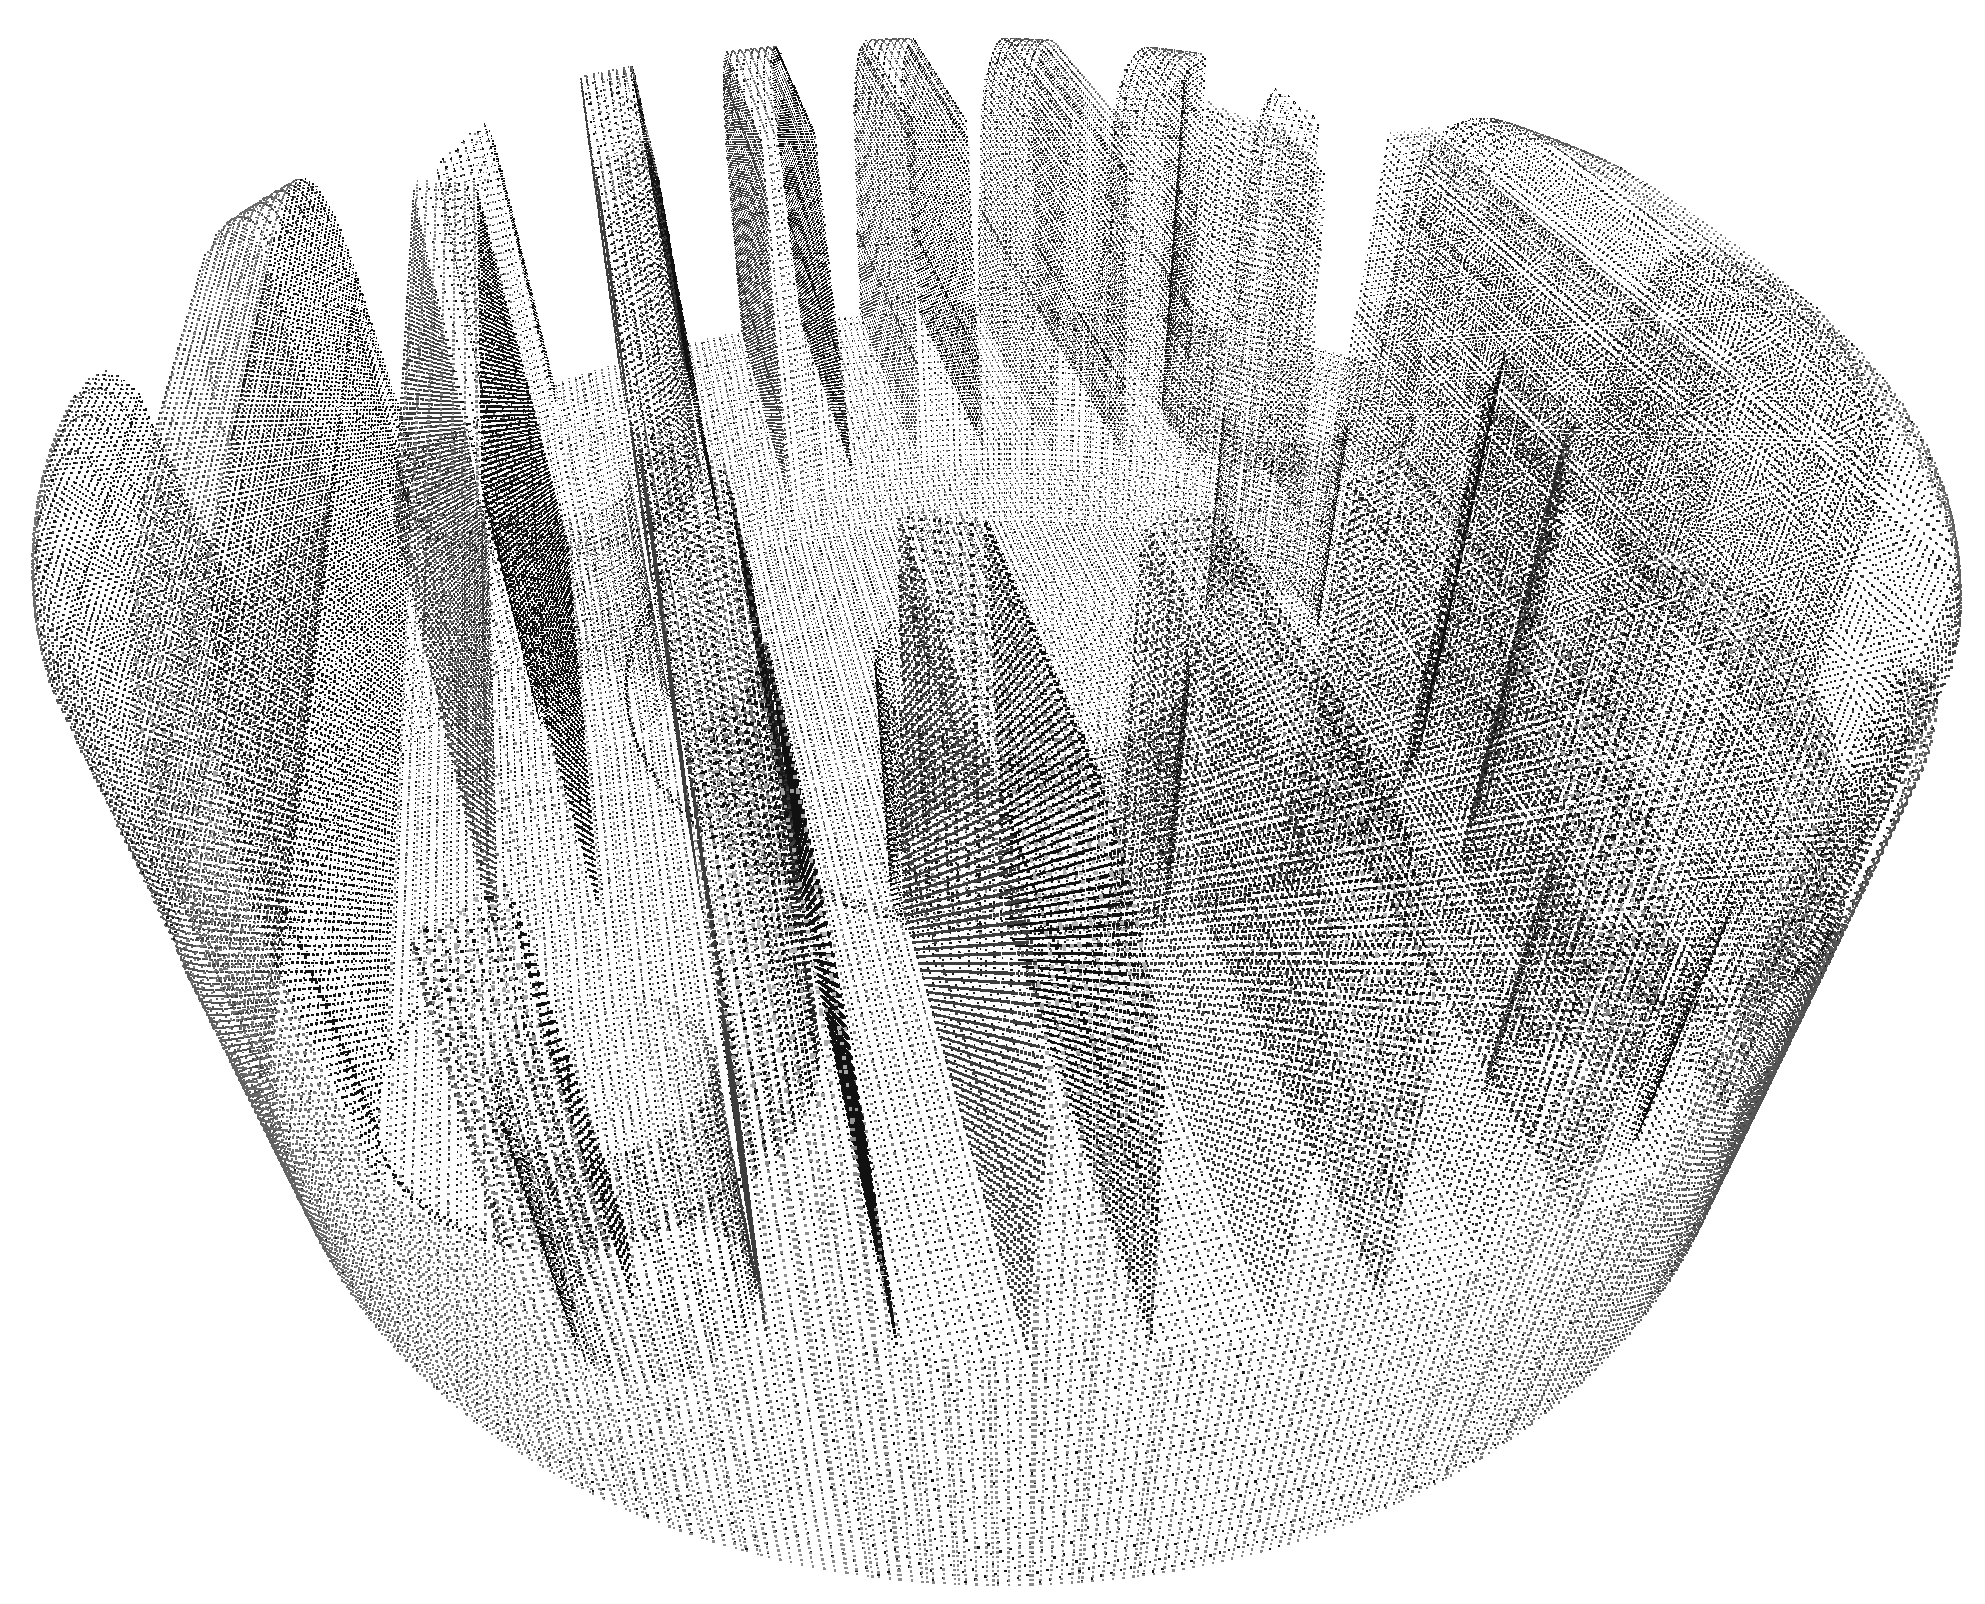
\includegraphics[width=\textwidth]{images/cylinder_head_point_cloud}
		\caption{cylinder\_head}
		\label{fig:cylinder_head_point_cloud_}
	\end{subfigure}
	\begin{subfigure}[t]{0.49\textwidth}
		\centering
		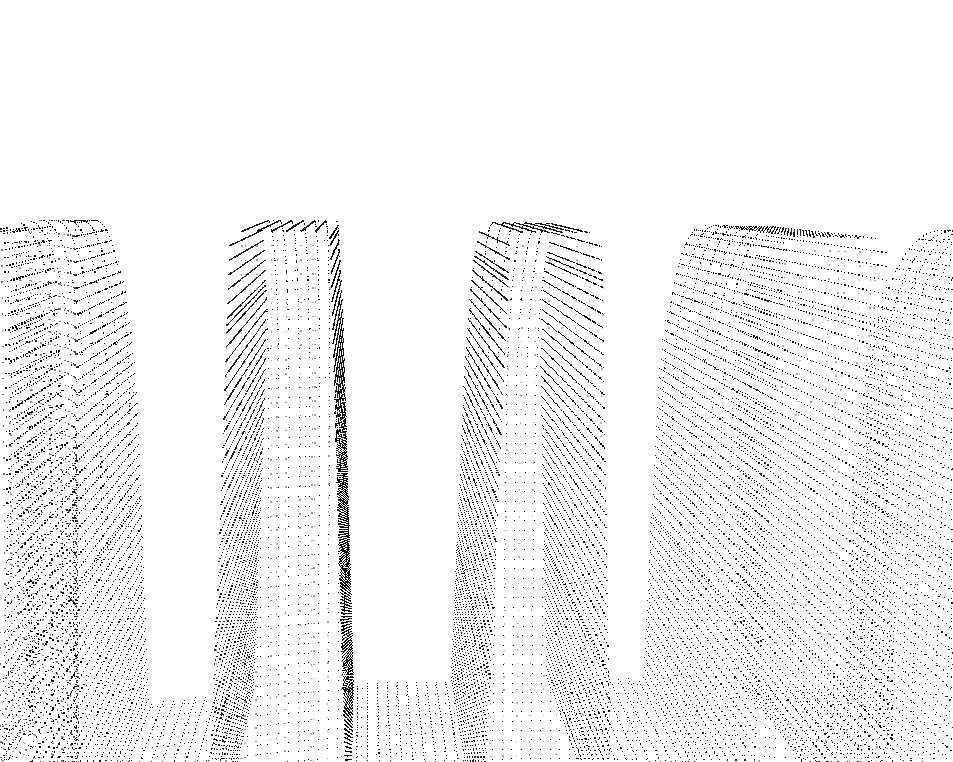
\includegraphics[width=\textwidth]{images/cylinder_head_point_cloud_fins}
		\caption{fins}
		\label{fig:cylinder_head_point_cloud_fins}
	\end{subfigure}
	\caption{
		Point cloud created by raycasting the cylinder\_head scene using three axis-aligned raycasts along the coordinate system's axes with a resolution of 200.
	}
	\label{fig:cylinder_head_point_cloud}
\end{figure}
%
Secondly, after the point cloud has been created, a surface reconstruction algorithm is run on it.

Regarding its quality, a point cloud sampled from the VML's regular grid using a uniform, axis-aligned raycast has a few properties:
\begin{itemize}
	\item
	All surface points, excluding numeric errors, are usually perfect samples, lying directly on the workpiece's surface.
	There is neither noise on the surface nor are there irrelevant inner or outer points.
	\item
	Each surface sample provides a perfect surface normal.
	\item
	The regularity of the raycaster guarantees a minimum and maximum density of the cloud, which may be derived from the distances between adjacent rays along each axis.
\end{itemize}

Despite these quality guarantees, a point cloud is still less rich in semantics when compared with a tri-dexel image.
The most prominent differences and commonalities are:
\begin{itemize}
	\item
	Point clouds only store surface information, whereas a tri-dexel image also holds volumetric information, \ie the dexel segments and point occupancy of the tri-dexel grid.
	\item
	Although a sufficient density is necessary, point clouds do not profit from the regular and uniform sampling.
	This property is fundamental for the tri-dexel approach, as it enables the construction of the regular tri-dexel grid and breaks down the problem of triangulation.
	\item
	The regularization of the tri-dexel cells provides a good way of detecting feature-rich regions which should be resampled with increased density.
	Such regions are harder to find within a point cloud, although local point distance and normal variance might give good hints.
	\item
	Although no regularization step is needed for small peculiarities of the cloud, it depends solely on the used reconstruction algorithm whether such small features are extracted or left unused.
	Regarding the tri-dexel approach presented in \cref{ch:tri_dexel}, such behavior is well-defined by either regularizing, \ie dropping, or slicing a cell with small features.
	\item
	Regarding both data structures, features which are not discovered by the raycaster are not present in the built data structures.
	Subsequent algorithms have to implement some kind of feature reconstruction.
	\item
	Point clouds are simpler data structures and easier to exchange with other 3D software.
	\item
	Point clouds have a substantially smaller memory footprint than tri-dexel images.
\end{itemize}


\section{Implementation}
\label{sec:point_cloud_implementation}

Reusing the axis-aligned raycast from \cref{sec:tri_dexel_raycast}, all reported surface intersections are just accumulated into a set of points.
Afterwards, any kind of surface reconstruction algorithm may used to proceed.

\subsection{Point cloud creation}
\label{sec:point_cloud_creation}

\Cref{alg:point_cloud_based} shows the basic routine used to obtain a point cloud and call a subsequent reconstruction algorithm.
%
\begin{algorithm}
	\centering
	\begin{algorithmic}[1]
		\Function{PointCloudBased}{$\var{grid}, \var{resolution}$}
			\State $\var{res} = \Call{UniformResolution}{\var{grid}.\var{aabb}, \var{resolution}}$
			\State $\var{cloud} = \varnothing$
			\State $\Call{AxisParallelRaycast}{\var{grid}, \var{grid}.\var{aabb}, \var{res},\hfill\break
				\hspace*{\dimexpr\algorithmicindent*2}(\var{\_}, \var{\_}, \var{\_}, \var{v}, \var{n}) \rightarrow \var{cloud}.\var{add}((\var{v}, \var{n}))}$
			\State \Return $\Call{ReconstructFromPointCloud}{\var{cloud}}$
		\EndFunction
	\end{algorithmic}
	\caption{
		Abstract workflow of the surface reconstruction using an arbitrary point cloud reconstruction algorithm \textproc{ReconstructFromPointCloud}.
	}
	\label{alg:point_cloud_based}
\end{algorithm}
%
Using the \textproc{UniformResolution} function, the algorithm starts off by computing an appropriate raycasting resolution \var{res} for all three axes, based on the \var{resolution} parameter passed by the user.
This step is also done before the tri-dexel raycast, but with an increased bounding box, \cf \cref{alg:tri_dexel}.
For the details of \textproc{UniformResolution} \cf \cref{sec:tri_dexel_implementation}.
Afterwards, an empty set of points, \var{cloud}, is created, which will accumulate all surface points emitted by the raycaster.
Afterwards, the raycast is launched with the calculated resolution and the grid's bounding box.
The closure passed to the raycasting subroutine \textproc{AxisParallelRaycast} is called at every surface hit with a list of arguments.
From these arguments only the last two, the intersection point \var{v} and the corresponding surface normal \var{n}, are relevant.
These two are added as tuple to the current point cloud \var{cloud}.
Mind that the closure is invoked concurrently, requiring $\var{cloud}.\var{add}$ to be thread-safe.
After the raycast has finished, a point cloud based surface reconstruction algorithm is run, indicated by the call to \textproc{ReconstructFromPointCloud}.

\subsection{Surface reconstruction}
\label{sec:point_cloud_reconstruction}

Two examples of algorithms for surface reconstruction from point clouds are given in the following:

\begin{description}
	\begin{figure}
		\centering
		\begin{subfigure}[b]{0.30\textwidth}
			\centering
			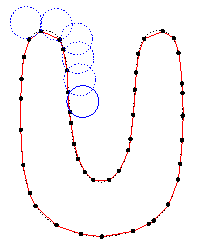
\includegraphics[width=\textwidth]{bpa_principle_1}
			\caption{
				Pivoting
			}
			\label{fig:bpa_principle_1}
		\end{subfigure}
		\begin{subfigure}[b]{0.30\textwidth}
			\centering
			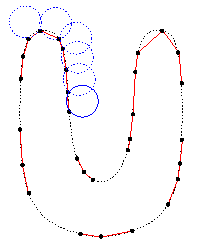
\includegraphics[width=\textwidth]{bpa_principle_2}
			\caption{
				Hole creation
			}
			\label{fig:bpa_principle_2}
		\end{subfigure}
		\begin{subfigure}[b]{0.30\textwidth}
			\centering
			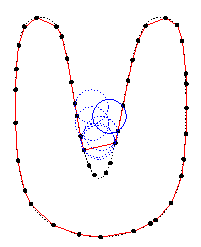
\includegraphics[width=\textwidth]{bpa_principle_3}
			\caption{
				Lost features
			}
			\label{fig:bpa_principle_3}
		\end{subfigure}
		\caption{
			Principle of the BPA surface reconstruction approach \cite{bpa}.
		}
		\label{fig:bpa_principle}
	\end{figure}

	\item[Ball pivoting algorithm] \hfill \\
	The ball pivoting algorithm (BPA) is a region growing algorithm, \cf \cref{fig:bpa_principle}.
	As the name suggests, it places a ball, \ie sphere, at the outside of the point cloud, touching three points, creating a seed triangle.
	From this seed triangle, the ball is pivoted over each edge of the triangle until it touches another point, creating a new triangle with new edges to roll over.
	If no point is found during pivoting, the edge is left as a boundary.
	The front of edges is rolled over repeatedly until no more edges are available.
	If all pivots where successful, a closed, manifold and oriented mesh has been created.
	The BPA requires a user supplied ball size, which steers the capability of rolling into finer features and the danger of creating holes or falling into the point cloud.
	If the point density is too low or the ball is too small, holes are created, \cf \cref{fig:bpa_principle_2}.
	If concave features are too small or the ball is too large, features may be lost, \cf \cref{fig:bpa_principle_3}.

	A highly tuned version of the BPA with elements of the G2S algorithm is already utilized by the VML for its swept volume computation \cite{bpa_vml}.
	A further implementation of the BPA is available in CGAL \cite{cgal_bpa}.
	MeshLab also offers a BPA version, parameterizable via its GUI.
	The BPA will be the main example for a point cloud surface reconstruction algorithm throughout this chapter, especially the results \cref{sec:point_cloud_results}.

%	\begin{figure}
%		\centering
%		\begin{subfigure}[b]{0.30\textwidth}
%			\centering
%			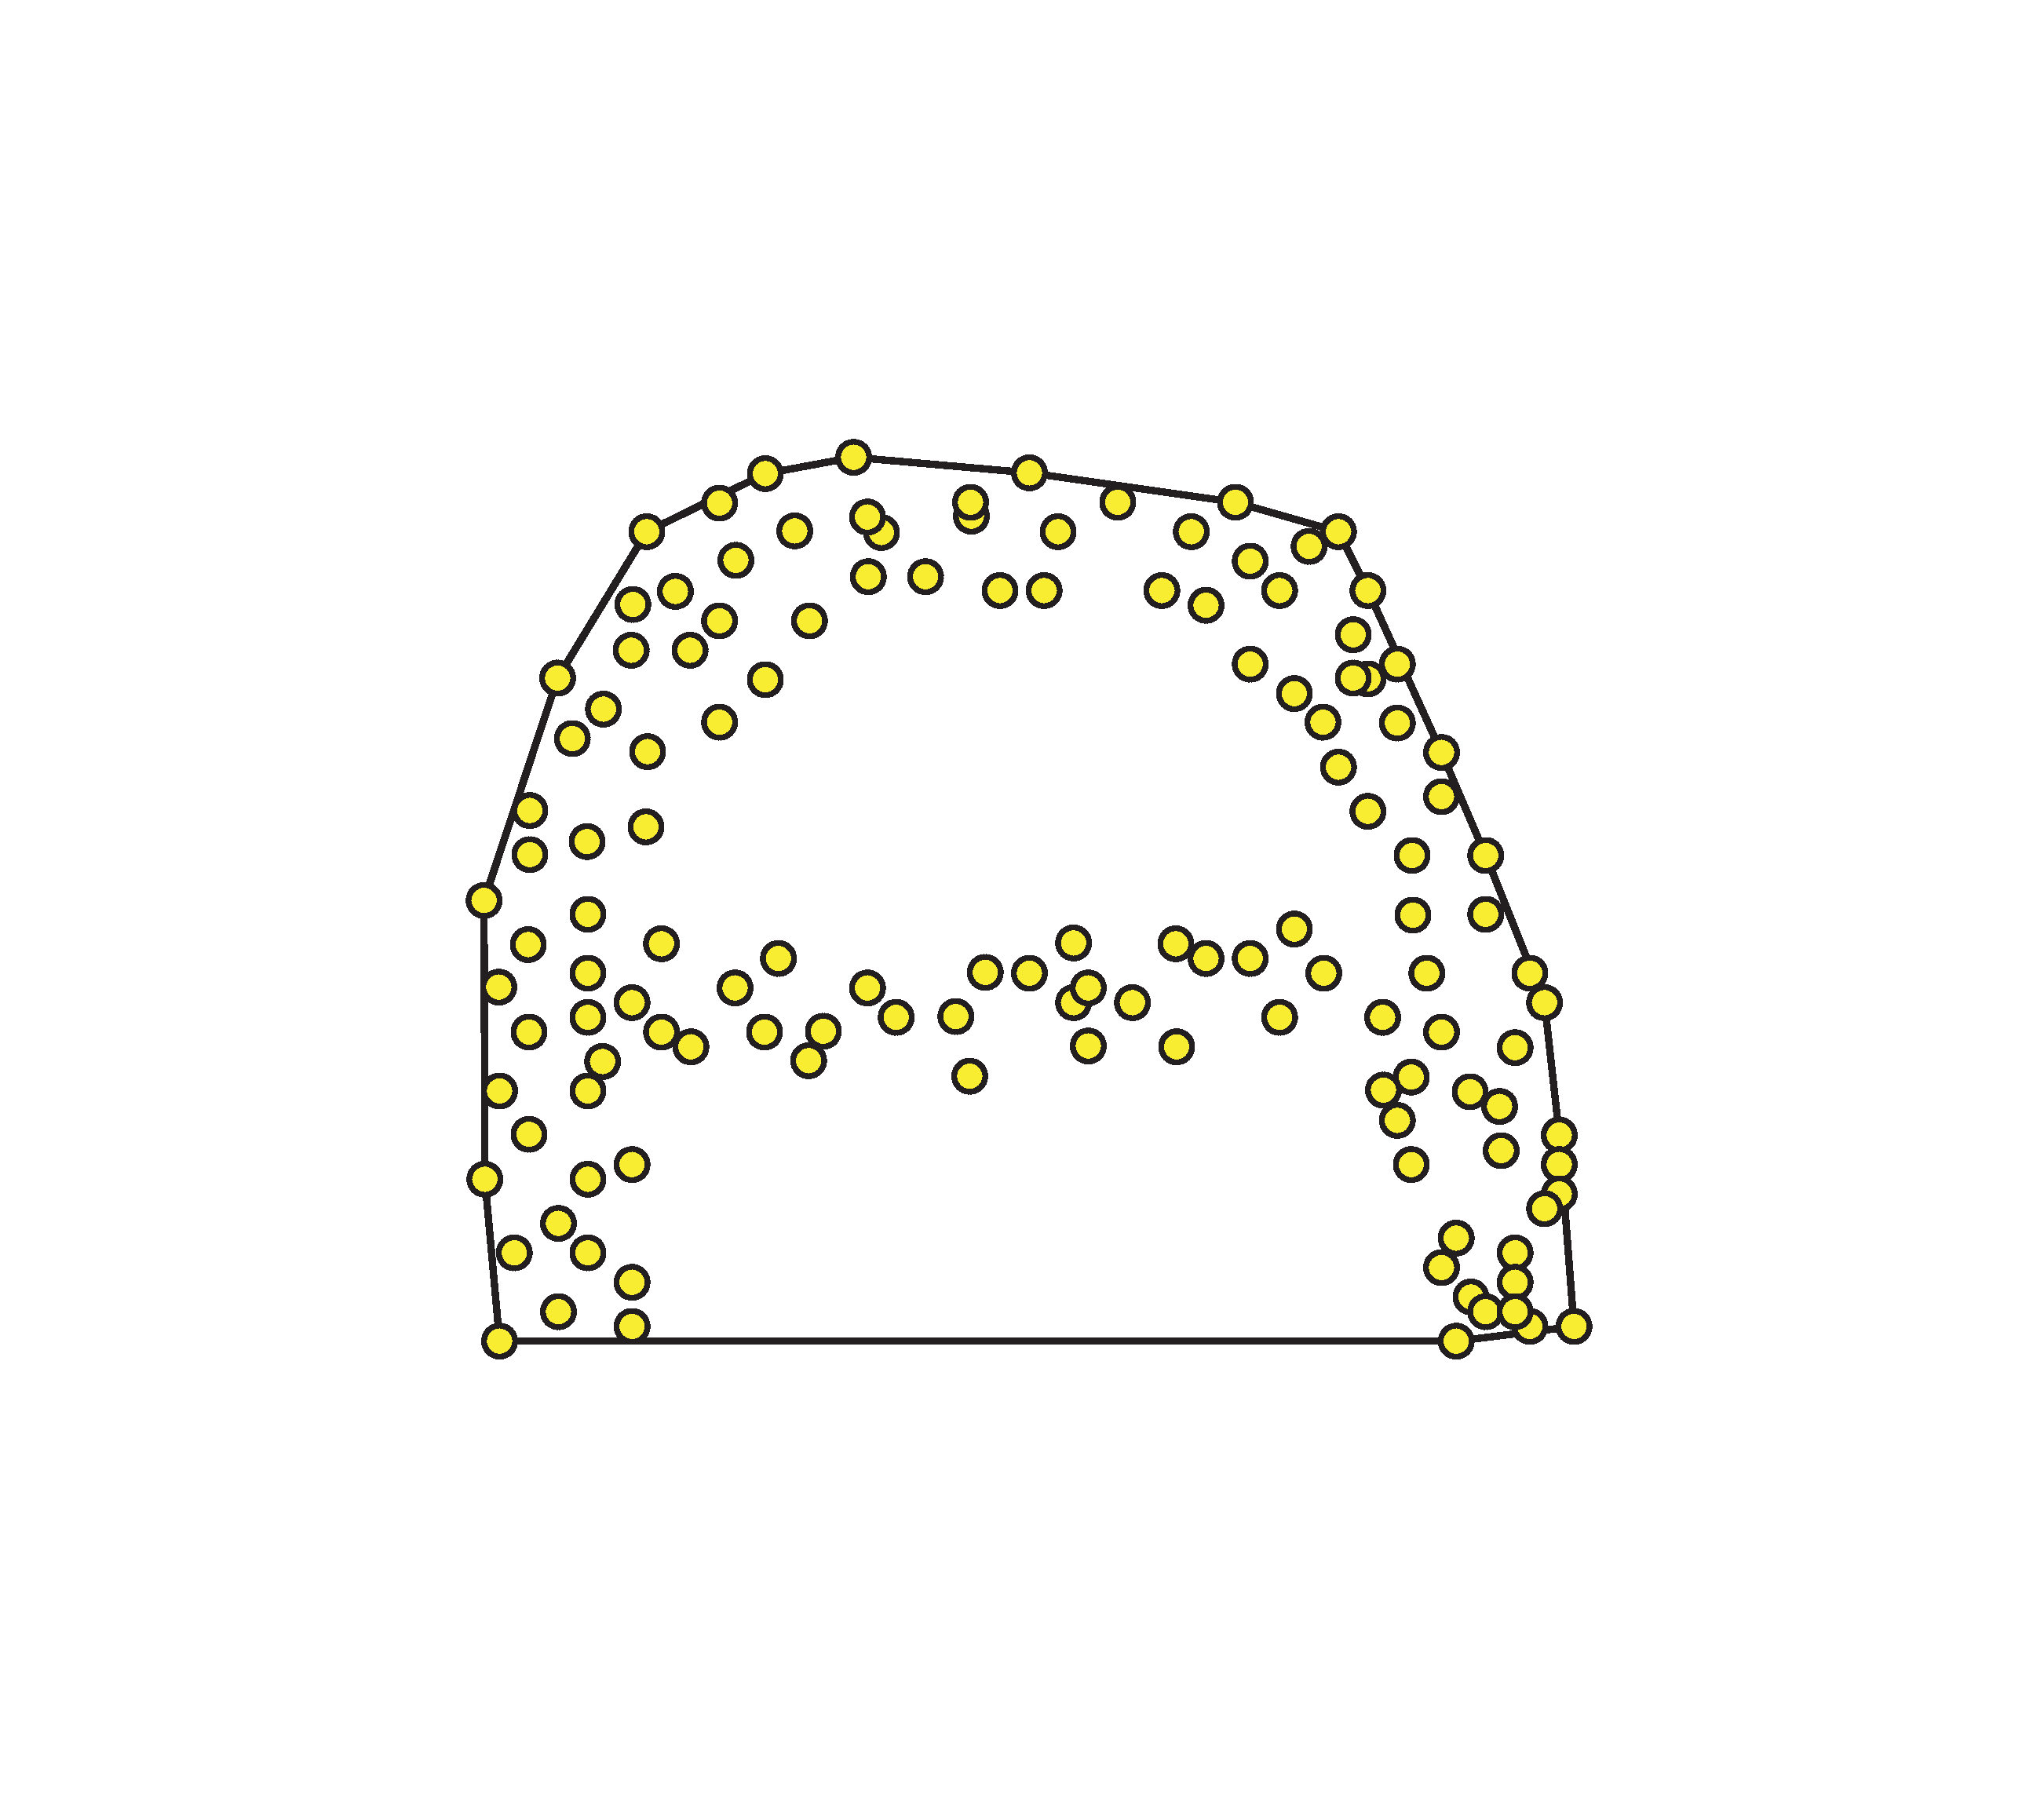
\includegraphics[width=\textwidth]{alpha_shapes_convex_hull}
%			\caption{
%				$\alpha = \infty$
%			}
%			\label{fig:alpha_shapes_convex_hull}
%		\end{subfigure}
%		\begin{subfigure}[b]{0.30\textwidth}
%			\centering
%			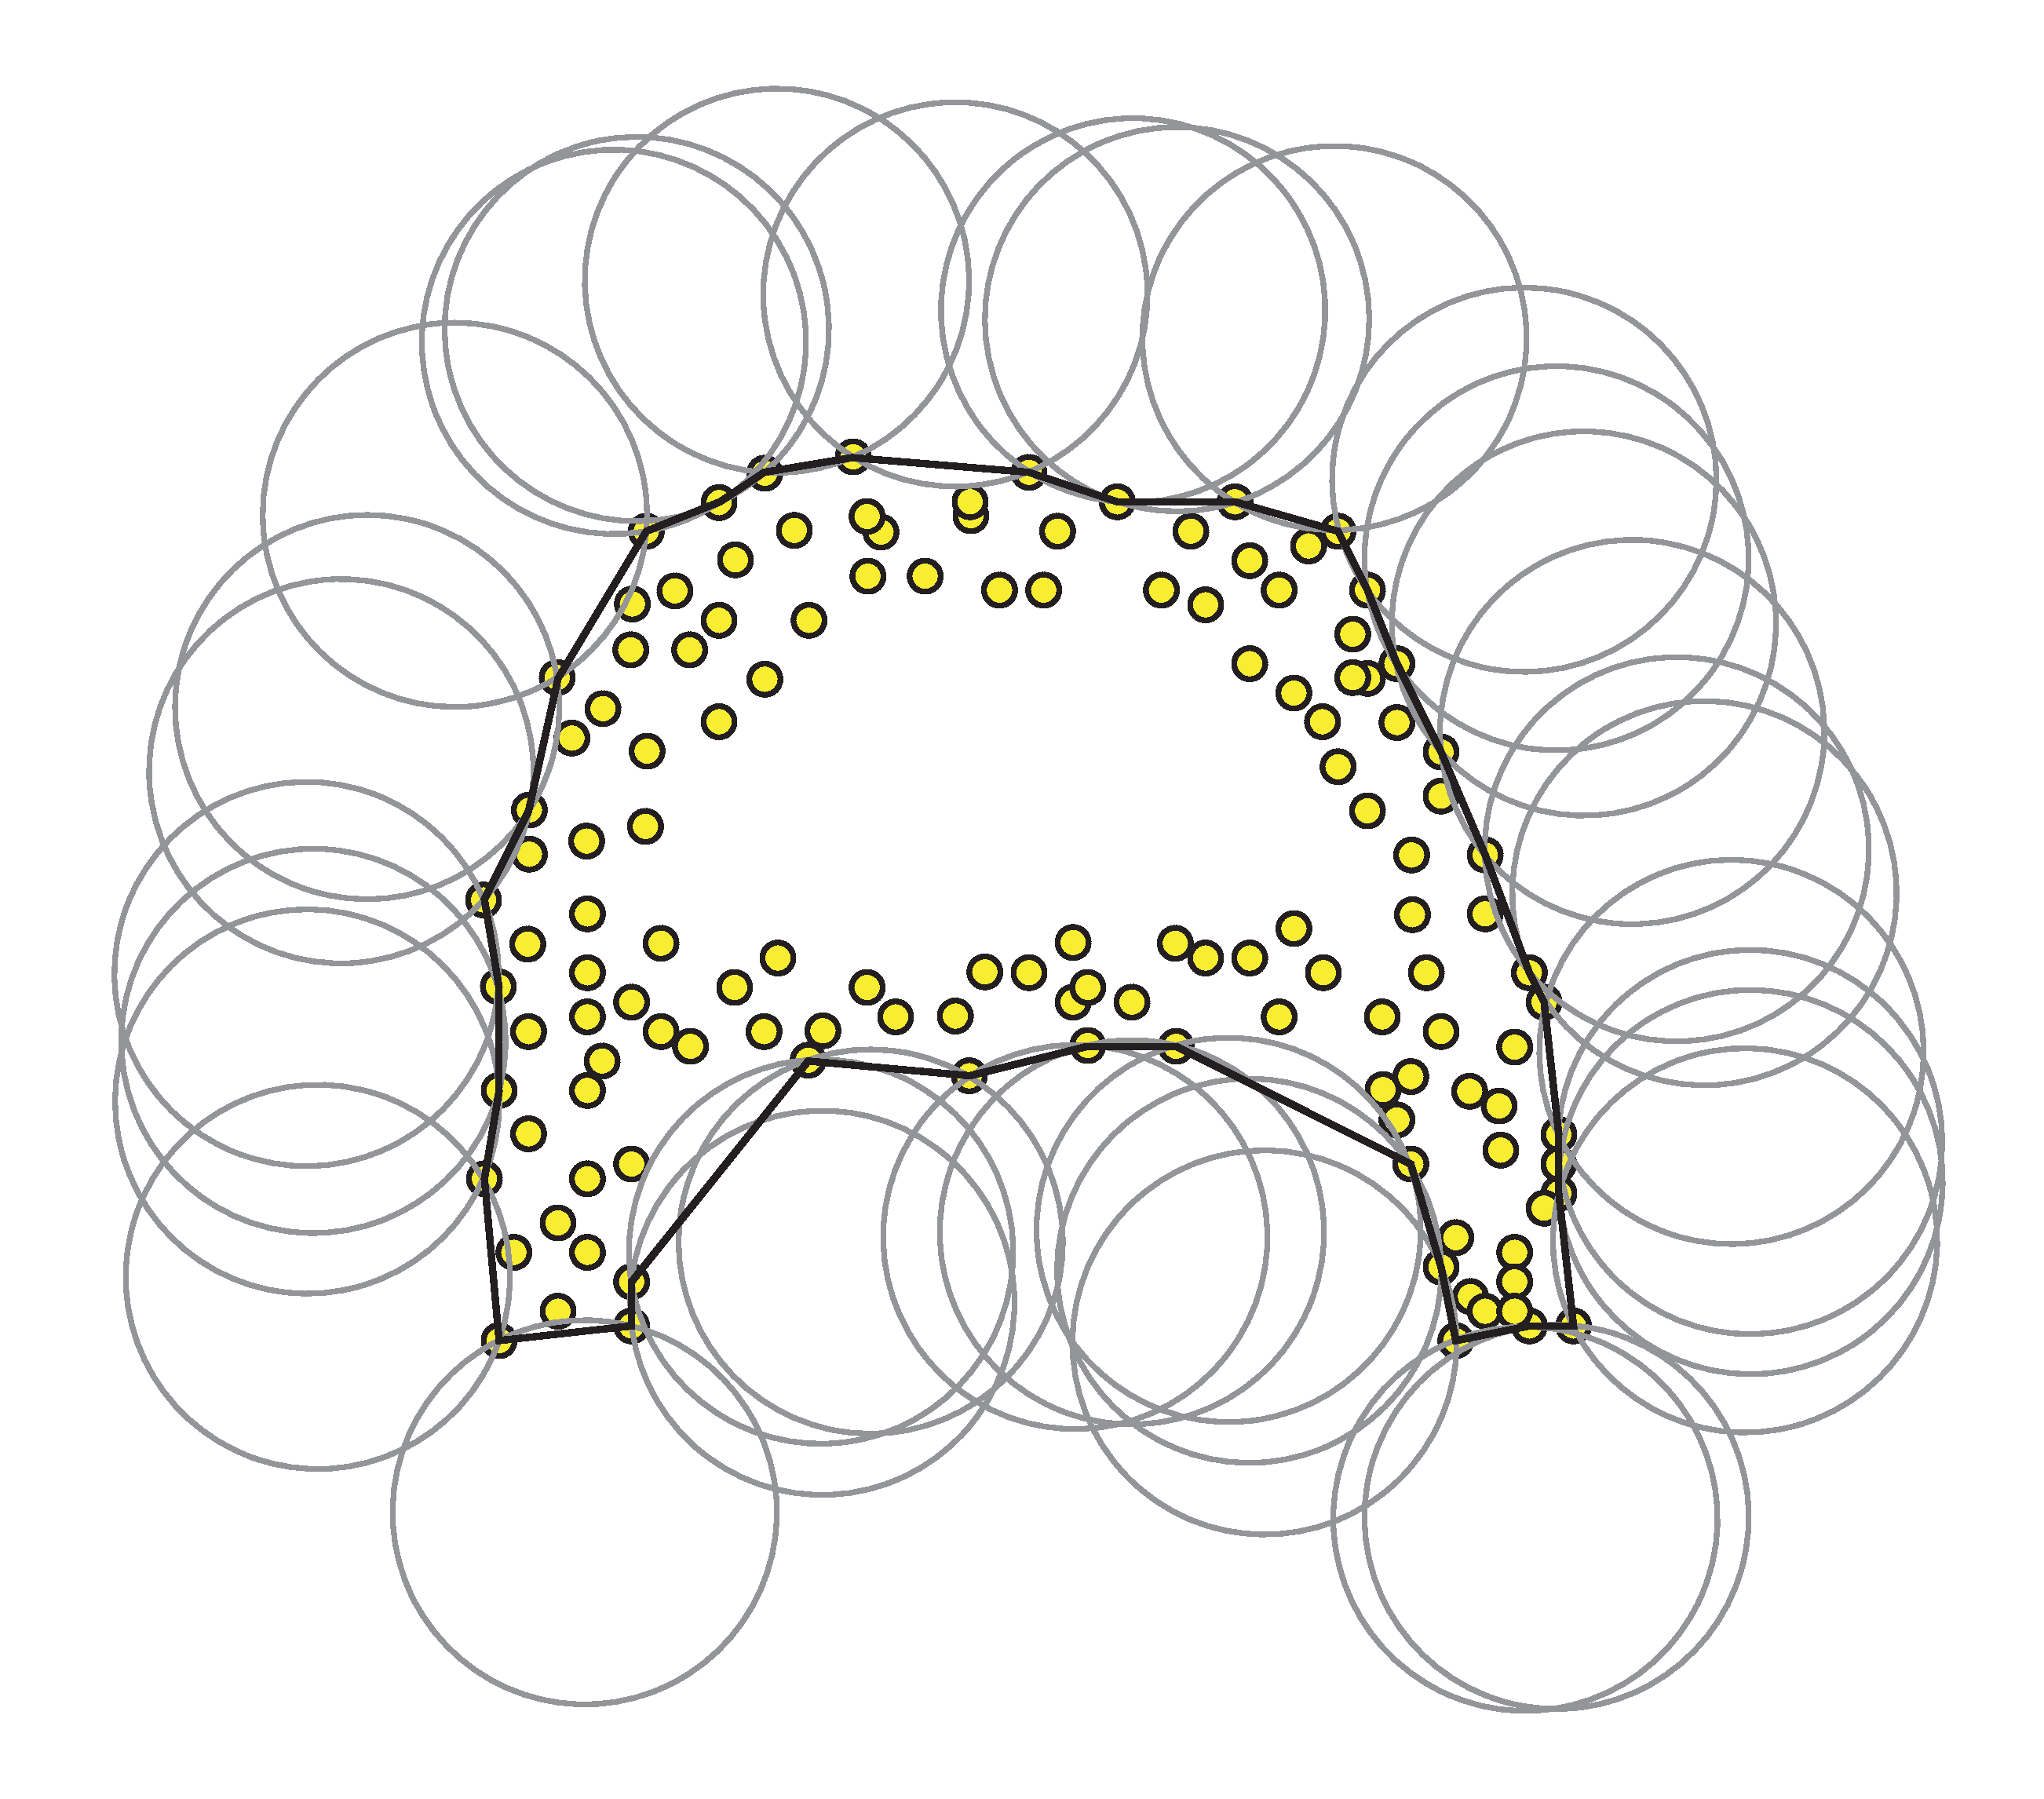
\includegraphics[width=\textwidth]{alpha_shapes_big_alpha}
%			\caption{
%				Big $\alpha$
%			}
%			\label{fig:alpha_shapes_big_alpha}
%		\end{subfigure}
%		\begin{subfigure}[b]{0.30\textwidth}
%			\centering
%			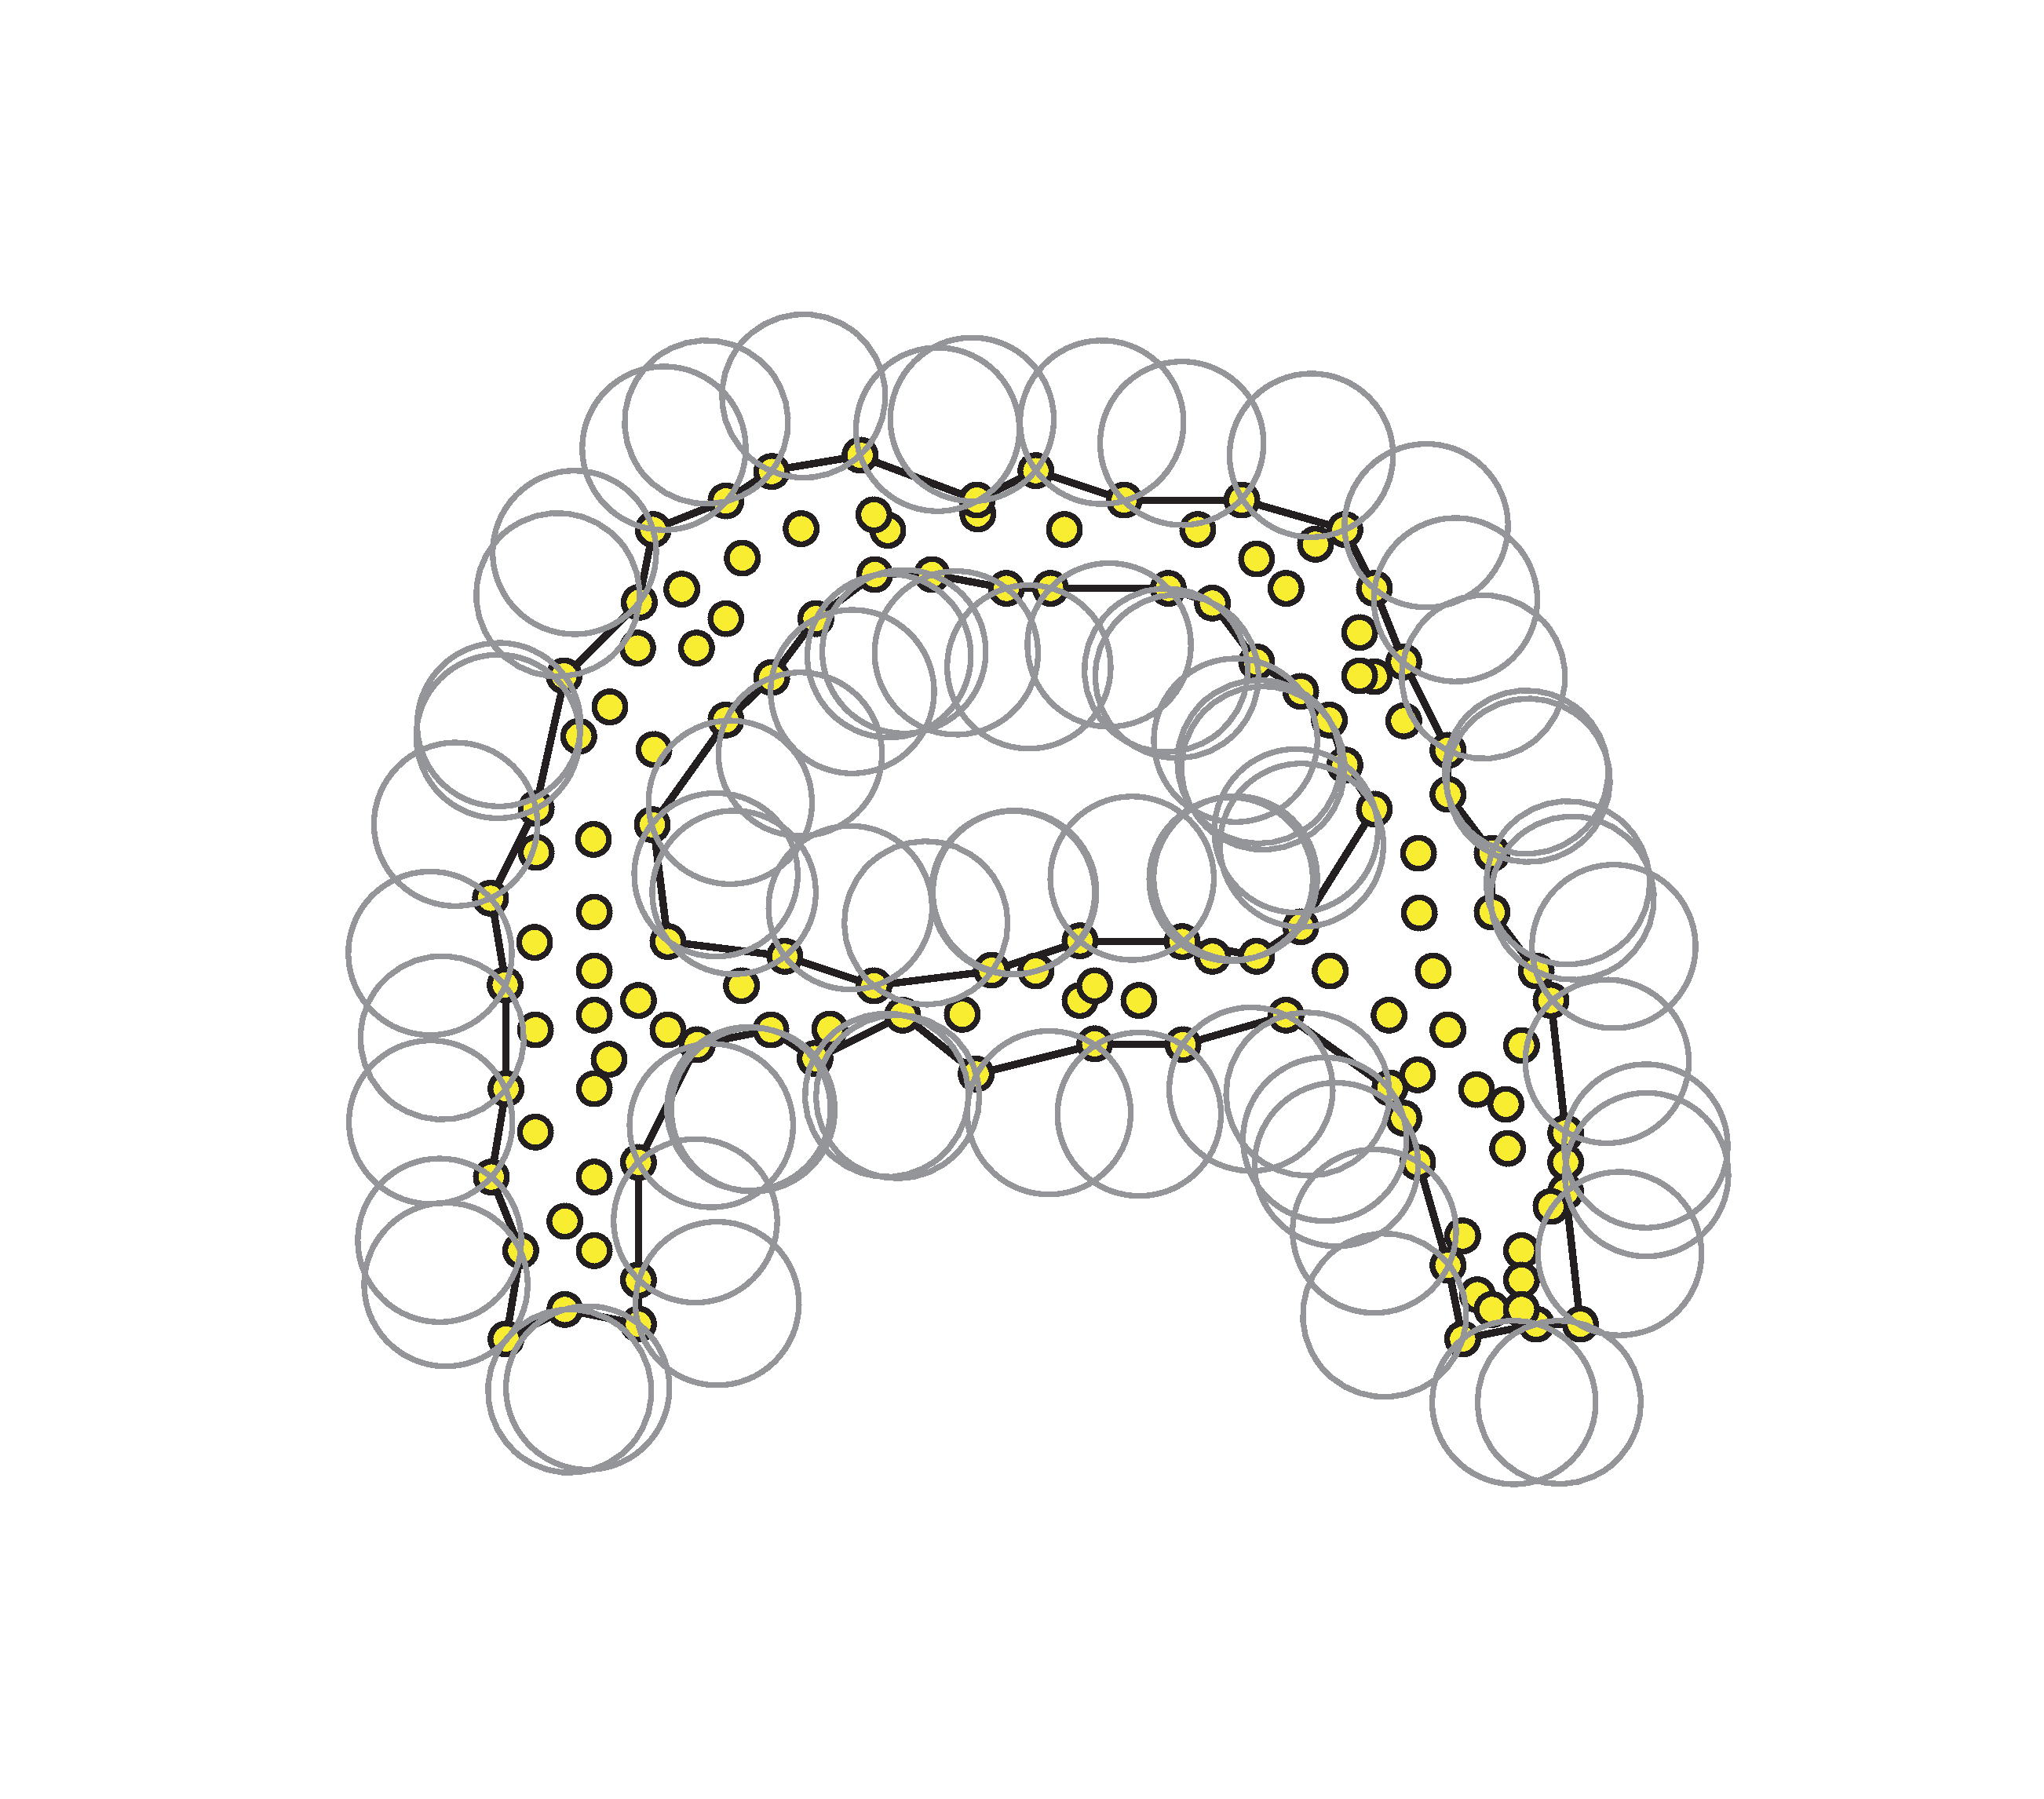
\includegraphics[width=\textwidth]{alpha_shapes_small_alpha}
%			\caption{
%				Small $\alpha$
%			}
%			\label{fig:alpha_shapes_small_alpha}
%		\end{subfigure}
%		\caption{
%			Principle of the alpha shapes surface reconstruction approach.
%			Based on \cite{alpha_shapes_images}.
%		}
%		\label{fig:alpha_shapes_principle}
%	\end{figure}
%
%	\item[$\alpha$-shape] \hfill \\
%	The $\alpha$-shape was one of the first tries to define a \enquote{shape} for a set of finite points \cite{alpha_shape}.
%	The $\alpha$-shape of a 3-dimensional point cloud is a set of triangles, where each triangle has at least one empty circumsphere with radius $\alpha$, \cf \cref{fig:alpha_shapes_principle}
%	It is quite similar to the BPA, but formulated statically, as no ball is rolled along the surface.
%	The $\alpha$-shape therefore also contains triangles within the point cloud, which would not be discovered by the BPA if the ball never rolls \enquote{inside} the point cloud, \ie sufficient density is given.
%	If $\alpha$ becomes $\infty$, the $\alpha$-shape becomes the convex hull of the point cloud, \cf \cref{fig:alpha_shapes_convex_hull}.
%	The magnitude of $\alpha$ determines
%	The empty circumsphere criterion further guarantees the triangulation to be a Delaunay triangulation, \ie the $\alpha$-shape is a subset of the 3-dimensional Delaunay triangulation.
%	An implementation of an $\alpha$-shape constructing algorithm is found in \eg the CGAL \cite{cgal_3d_alpha_shapes}, VTK \cite{vtk}, QHull \cite{qhull} or PCL \cite{pcl} library.
%	MeshLab provides user-friendly access the QHull version of the algorithm via a GUI.

	\begin{figure}
		\centering
		\begin{subfigure}[b]{0.24\textwidth}
			\centering
			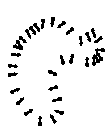
\includegraphics[width=\textwidth]{poisson_oriented_points}
			\captionsetup{justification=centering}
			\caption{
				oriented points\\
				$V$
			}
			\label{fig:poisson_oriented_points}
		\end{subfigure}
		\begin{subfigure}[b]{0.24\textwidth}
			\centering
			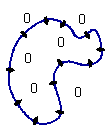
\includegraphics[width=\textwidth]{poisson_gradient_function}
			\captionsetup{justification=centering}
			\caption{
				indicator gradient\\
				$\nabla\chi$
			}
			\label{fig:poisson_gradient_function}
		\end{subfigure}
		\begin{subfigure}[b]{0.24\textwidth}
			\centering
			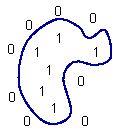
\includegraphics[width=\textwidth]{poisson_indicator_function}
			\captionsetup{justification=centering}
			\caption{
				indicator\\
				$\chi$
			}
			\label{fig:poisson_indicator_function}
		\end{subfigure}
		\begin{subfigure}[b]{0.24\textwidth}
			\centering
			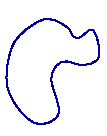
\includegraphics[width=\textwidth]{poisson_surface}
			\captionsetup{justification=centering}
			\caption{
				surface\\
				~
			}
			\label{fig:poisson_surface}
		\end{subfigure}
		\caption{
			Principle of the Poisson surface reconstruction approach \cite{poisson}.
		}
		\label{fig:poisson_principle}
	\end{figure}

	\item[Poisson] \hfill \\
	Poisson surface reconstruction is based on implicit functions \cite{poisson}, \cf \cref{fig:poisson_principle}.
	The goal is to compute a so-called indicator function $\chi$, which yields one for positions inside the workpiece and zero for positions outside, \cf \cref{fig:poisson_indicator_function}
	When moving into the workpiece from outside, the values of $\chi$ change from zero to one around the surface.
	The indicator function $\chi$, specifically its gradient $\nabla\chi$, \cf \cref{fig:poisson_gradient_function}, is strongly related to the normals of the input point set, a vector field $V$, \cf \cref{fig:poisson_oriented_points}.
	Therefore, the problem becomes finding a function $\chi$ whose gradient $\nabla\chi$ best approximates $V$, the normals of the point cloud, \ie $\min_\chi |\nabla\chi - V|$.
	This problem is then transformed into a standard Poisson problem, further details are given in the corresponding work \cite{poisson}.
	For the computation of these functions, the problem space is partitioned using an octree, whose depth provides the main variable to balance memory/computational demands and reconstruction quality.
	The reconstruction of a surface is finally done by extracting an isosurface of $\chi$.

	Implementations of Poisson surface reconstruction are found in \eg the CGAL \cite{cgal_poisson}, VTK \cite{vtk_poisson} and PCL \cite{pcl} library.
	MeshLab also integrates a Poisson implementation into its GUI.
\end{description}
